% Pappus: A, B, C and A', B', C' on two lines; X = AB'.A'B, Y = AC'.A'C, Z = BC'.B'C are collinear.
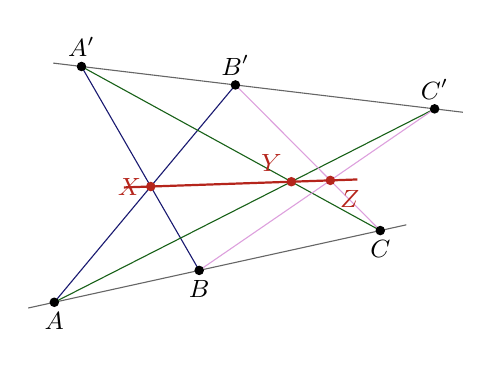
\begin{tikzpicture}[scale=1.15,font=\small]
\draw[black!60] (-0.2880,-0.0634) -- (3.8880,0.8554);
\draw[black!60] (-0.0120,2.6414) -- (4.5120,2.0986);
\draw[MidnightBlue] (0.0000,0.0000) -- (2.0000,2.4000);
\draw[MidnightBlue] (0.3000,2.6040) -- (1.6000,0.3520);
\draw[ForestGreen!70!black] (0.0000,0.0000) -- (4.2000,2.1360);
\draw[ForestGreen!70!black] (0.3000,2.6040) -- (3.6000,0.7920);
\draw[Plum] (1.6000,0.3520) -- (4.2000,2.1360);
\draw[Plum] (2.0000,2.4000) -- (3.6000,0.7920);
\draw[BrickRed,thick] (0.7678,1.2682) -- (3.3462,1.3562);
\fill[black] (0.0000,0.0000) circle (1.5pt) node[below,black] {$A$};
\fill[black] (1.6000,0.3520) circle (1.5pt) node[below,black] {$B$};
\fill[black] (3.6000,0.7920) circle (1.5pt) node[below,black] {$C$};
\fill[black] (0.3000,2.6040) circle (1.5pt) node[above,black] {$A'$};
\fill[black] (2.0000,2.4000) circle (1.5pt) node[above,black] {$B'$};
\fill[black] (4.2000,2.1360) circle (1.5pt) node[above,black] {$C'$};
\fill[BrickRed] (1.0653,1.2783) circle (1.5pt) node[left,BrickRed] {$X$};
\fill[BrickRed] (2.6178,1.3313) circle (1.5pt) node[above left,BrickRed] {$Y$};
\fill[BrickRed] (3.0487,1.3460) circle (1.5pt) node[below right,BrickRed] {$Z$};
\end{tikzpicture}
